\chapter{Implementacija i korisničko sučelje}
		
		
		\section{Korištene tehnologije i alati}
			
			\textnormal{
			Timski rad na ovom projektu zahtjeva konstanto surađivanje i praćenje
			stupnja razvijenosti aplikacije u procesu razvoja. Stoga je kao sustav za praćenje razvoja aplikacije korišten git. Git se sastoji od udaljenog, zajedničkog repozitorija, pohranjenog na poslužitelju GitLab, i lokalnih repozitorija svakog timskog člana što osigurava kontinuirano praćenje napretka, te na taj način svi imaju uvid u najnovije stanje i promjene dokumentacije i izvornoga koda aplikacije.}
		
			\smallbreak
			
			\textnormal{
			Za izradu dokumentacije korišten je programski jezik LaTeX. Za
			razliku od ostalih poznatih uređivača teksta LaTeX dopušta surađivanje sustavom Git. Dokumentacija je pisana u uređivačkom programu TeXstudio, a odabrani prevoditelj je texLive. Dijagrami su napravljeni u uređivačkom programu Astah Professional, a u dokumentaciju su uvezeni kao .png slike generirane is Astah programa.}
		
			\smallbreak
			
			\textnormal{
			Za razvojno okruženje odabran je Microsoft Visual Studio, tvrtke
			Microsoft. Za radni okvir aplikacije odabran je ASP.NET Core koji podržava razvoj web aplikacija uključujući web servise, web resurse i web API-je. Razvojni model aplikacije je MVC (Model, View, Controller).
			Datoteke View komponente (frontend) su pisane u prezentacijskom jeziku HTML, stilskom jeziku CSS i skriptnom programskom jeziku JavaScript.
			Za kreiranje reaktivnih stranica (single-page applications, SPA) i korisničkih sučelja u frontendu korišten je Vue.js javascript okvir.
			Za pisanje datoteka u komponentama Model i Controller (backend) korišten je programski jezik C\#.
			Baza podataka se nalazi na poslužitelju u oblaku Microsoft Azure.\\
			\\
			\url{https://git-scm.com/}\\
			\url{https://gitlab.com/}\\
			\url{https://www.latex-project.org/}\\
			\url{http://astah.net/editions/professional}\\
			\url{https://visualstudio.microsoft.com/}\\
			\url{https://docs.microsoft.com/en-us/aspnet/core/?view=aspnetcore-3.1}\\
			\url{https://docs.microsoft.com/en-us/dotnet/csharp/}\\
			\url{https://www.javascript.com/}\\
			\url{https://portal.azure.com/}\\
			\url{https://vuejs.org/}}
			
			
			\eject 
		
	
		\section{Ispitivanje programskog rješenja}
			
			\textbf{\textit{dio 2. revizije}}\\
			
			 \textnormal{Popularni pristup razvoju testiranja (TDD) je pisanje testa prije implementacije ciljanog koda.  	Testiranje aplikacija postalo je uobičajena praksa za današnje softvere, a xUnit je jedan od najpopularnijih okvira za testiranje jedinica dostupan za .NET. Pisan je u jeziku C\#. U našoj aplikaciji smo također koristili xUnit te smo testiranja pisali po obrascima uporabe. Uvijek smo ponavljali isti pristup, pisali smo neuspjeli test i zatim ažurirali ciljni kod koji treba proći.Napisali smo 24 xUnit testa kako bismo testirali većinu naših obrazaca uporabe (za one jako jednostavne nisu ni bili potrebni testovi), no zbog jednostavnosti opisat ćemo samo tri integracijska testa.}
			 \bigbreak
			 \textnormal {	Prvi, jedan od najvažnijih testova, jest test prijave u sustav (UC3). Test prijave u sustav provjerava prijavu u svim ulogama: admin, trener, član uprave i kijent. Sastoji se od nekoliko funkcija u kojima se provjerava u bazi ispravnost korisničkog imena i lozinke. Na primjer, korisnik se ne može prijaviti s netočnom formom e-mail adrese. }
			 	\begin{packed_item}
			 	
			 	\item Prijava u sustav s e-mail adresom abc.com (pogrešna forma e-maila)
			 	\item[] \begin{packed_enum}
			 		\item očekivani ishod: aplikacija javi korisniku da e-mail nije dobro unesen e-mail i ne dozvoljava mu prijavu u sustav te nudi opciju da pokuša ponovno.
			 		\item očekivani ishod xUnit testa: test bi dao HTML odgovor da je prijava neuspjela
			 	\end{packed_enum}
			 \end{packed_item}
		 \textnormal {Ishod je bio kao što je i očekivano, odnosno test je prošao.}
		 
		 	\begin{packed_item}
		 	
		 	\item Prijava u sustav s netočnom lozinkom/e-mailom
		 	\item[] \begin{packed_enum}
		 		\item očekivani ishod: aplikacija javlja korisniku da mu je lozinka/mail pogrešan, odnosno da to nije važeći račun i onemogućava mu prijavu
		 		\item očekivani ishod xUnit testa: test vraća HTML odgovor o neuspjeloj prijavi
		 		
		 	\end{packed_enum}
		 \end{packed_item}
		 \textnormal {Ishod se i u ovom slučaju podudarao s očekivanim, odnosno test je ponovno prošao.}
		 \bigbreak
		 \textnormal {Drugi test koji ćemo spomenuti jest dohvaćanje postojećih objava. Test je osmišljen tako da korisnik mora biti ulogiran kao admin ili trener da bi mogao pristupiti objavama te provjerava za svaku pojedinačnu dohvaćenu objavu postoji li u bazi podataka te ako ne postoji, odnosno ako se prikazala pogrešna lista, vraća očekivanu poruku. Test je prošao.}
		 \bigbreak
		 \textnormal{Treći test je također vezan za objave, a može biti i za bilo koji dio baze podataka (slika, artikl, košarica). U tom se testu provjerava ispravno dohvaćanje, brisanje te traženje objave. Korisnik mora imati određenu razinu autorizacije, inače ne može tome pristupiti. Nakon što korisnik dohvati objavu, ako je dobro dohvaćena, može ju izbrisati i izbriše ju te joj pokuša ponovno pristupiti. Test bi trebao vraćati “Not found” status, odnosno ako baza ispravno radi, objava je iz nje izbrisana i ne može ju se dohvatiti. U ova se dva testa provjeravala ispravnost baze podataka. I ovaj je test prošao.
		 }
	
			
			\subsection{Ispitivanje komponenti}
			
			\textnormal{Ispitni slučajevi su testirani pomoću alata Selenium IDE. Određeni su redovni i rubni slučajevi koji opisuju moguće akcije korisnika na web aplikaciji.\\}
		 	
		 	\textnormal{\textbf{Ispitni slučaj 1: Interakcija s web-shopom i pregledavanje dostupnih artikala\\}}
		 	
		 	\textnormal{\textbf{Ulaz:}}
		 	
		 	\begin{packed_enum}
		 		\item Otvaranje početne stranice u web pregledniku.
		 		\item Otvaranje login stranice i unos e-maila i lozinke.
		 		\item Otvaranje stranice web-shopa.
		 		\item Pomicanje kotačića na mišu i pregledavanje artikala web-shopa.
		 		\item Klik na gumb artikla \textit{Dodaj u košaricu}.
		 		\item Otvaranje korisničke košarice.
		 		\item Klik na gumb brisanja artikla.
		 		\item Klik na gumb \textit{Isprazni košaricu}.
		 	\end{packed_enum}
	 	
	 		\textnormal{\textbf{Očekivani rezultat:}}
	 		
	 		\begin{packed_enum}
	 			\item Prikazuje se web-shop logiranog korisnika.
	 			\item Odabrani artikl se dodaje u košaricu.
	 			\item Otvaranje i prikaz košarice artikala.
	 			\item Brisanje jednog artikla.
	 			\item Brisanje svih artikala.
	 		\end{packed_enum}
 		
 			\textnormal{\textbf{Rezultat:}}
 			
 			\textnormal{Akcije pregledavanja web-shopa, dodavanja artikala u košaricu i brisanje artikala košarice su funkcionalne. \textcolor{green}{Aplikacija je prošla test.\\}}
 			
 			\textnormal{\textbf{Ispitni slučaj 2: Login korisnika}\\}
 			
 			\textnormal{\textbf{Ulaz:}}
 			
 			\begin{packed_enum}
 				\item Otvaranje početne stranice u web pregledniku.
 				\item Otvaranje login stranice.
 				\item Unos e-mail korisnika.
 				\item Unos lozinke korisnika.
 				\item Klik na gumb \textit{Login}.
 			\end{packed_enum}
 			
 			\textnormal{\textbf{Očekivani rezultat:}}
 			
 			\begin{packed_enum}
 				\item Otvaranje stranice login obrasca.
 				\item Unos i provjera korisničkih podataka u bazi podataka.
 				\item Prikaz početne stranice sa korisničim profilom u gornjem desnom kutu.
 			\end{packed_enum}
 			
 			\textnormal{\textbf{Rezultat:}}
 			
 			\textnormal{Prikaz login stranice i provjera unešenih podataka. \textcolor{green}{Aplikacija je prošla test.}\\}
 			
 			\textnormal{\textbf{Ispitni slučaj 3: Registracija korisnika}\\}
 			
 			\textnormal{\textbf{Ulaz:}}
 			
 			\begin{packed_enum}
 				\item Otvaranje početne stranice u web pregledniku.
 				\item Otvaranje stranice za registraciju.
 				\item Unos željenog e-mail korisnika.
 				\item Unos željene lozinke korisnika.
 				\item Popunjavanje ostalih podataka.
 				\item Klik na gumb \textit{Registriraj se}.
 			\end{packed_enum}
 			
 			\textnormal{\textbf{Očekivani rezultat:}}
 			
 			\begin{packed_enum}
 				\item Otvaranje stranice obrasca za registriranje.
 				\item Unos korisničkih podataka.
 				\item Zapis unešenih korisničkih podataka u bazi podataka.
 				\item Prikaz početne stranice sa korisničim profilom u gornjem desnom kutu.
 			\end{packed_enum}
 			
 			\textnormal{\textbf{Rezultat:}}
 			
 			\textnormal{Prikaz stranice za registraciju i zapis unešenih podataka u bazi podataka. \textcolor{green}{Aplikacija je prošla test.}\\}
 			
 			\textnormal{\textbf{Ispitni slučaj 4: Rubni slučaj prilikom korisničkog logina}\\}
 			
 			\textnormal{\textbf{Ulaz:}}
 			
 			\begin{packed_enum}
 				\item Otvaranje početne stranice web aplikacije.
 				\item Otvaranje stranice za login korisnika.
 				\item Nepotpun unos podataka (e-mail i/ili lozinka nedostaje) ili pogrešan unos.
 				\item Klik na gumb \textit{Login}.
 			\end{packed_enum}
 			
 			\textnormal{\textbf{Očekivani rezultat:}}
 			
 			\begin{packed_enum}
 				\item Otvaranje stranice login obrasca.
 				\item Nepotpun ili pogrešan unos podataka.
 				\item Klik na gumb \textit{Login}.
 				\item Ispis poruke upozorenja da određeni podatak mora biti unijet ili je pogrešan.
 			\end{packed_enum}
 			
 			\textnormal{\textbf{Rezultat:}}
 			
 			\textnormal{Korsnik dobiva obavijest da je unos podataka nepotpun ili pogrešan. \textcolor{green}{Aplikacija je prošla test.}}
			
			\eject 
		
		
		\section{Dijagram razmještaja}
			
			\textbf{\textit{dio 2. revizije}}
			
			 \textit{Potrebno je umetnuti \textbf{specifikacijski} dijagram razmještaja i opisati ga. Moguće je umjesto specifikacijskog dijagrama razmještaja umetnuti dijagram razmještaja instanci, pod uvjetom da taj dijagram bolje opisuje neki važniji dio sustava.}
			
			\eject 
		
		\section{Upute za puštanje u pogon}
		
			\textbf{\textit{dio 2. revizije}}\\
			 
			 \textnormal{Aplikacija je razvijena u okviru ASP.NET Core 3 uz korištenje SQL Server relacijske baze podataka. Prilikom izrade baze podataka koristili smo pristup "Database First". To znači da smo prvo konstruirali bazu, izgenerirali SQL kod za nju te pomoću .NET Core-a izgenerirali C\# razrede koji opisuju strukturu baze. Kako bismo osigurali da se aplikacija može spojiti na bazu, potrebno je u datoteci "appsettings.json" podesiti connection string na vrijednost: "\textit{Server=(localdb)\\mssqllocaldb;Database=RudesDatabase;Trusted\_Connection=True;}". Prilikom prvog pokretanja aplikacije, potrebno je ispuniti bazu podacima iz seeder razreda, a to se radi pomoću linije "\textit{RudesDatabaseSeeder.Initialize(app);}" u datoteci Startup.cs. Nakon toga, dovoljno je aplikaciju pokrenuti odabirom "Run" pa "Start without Debugging".}
			 
			 \begin{figure}[H]
			 	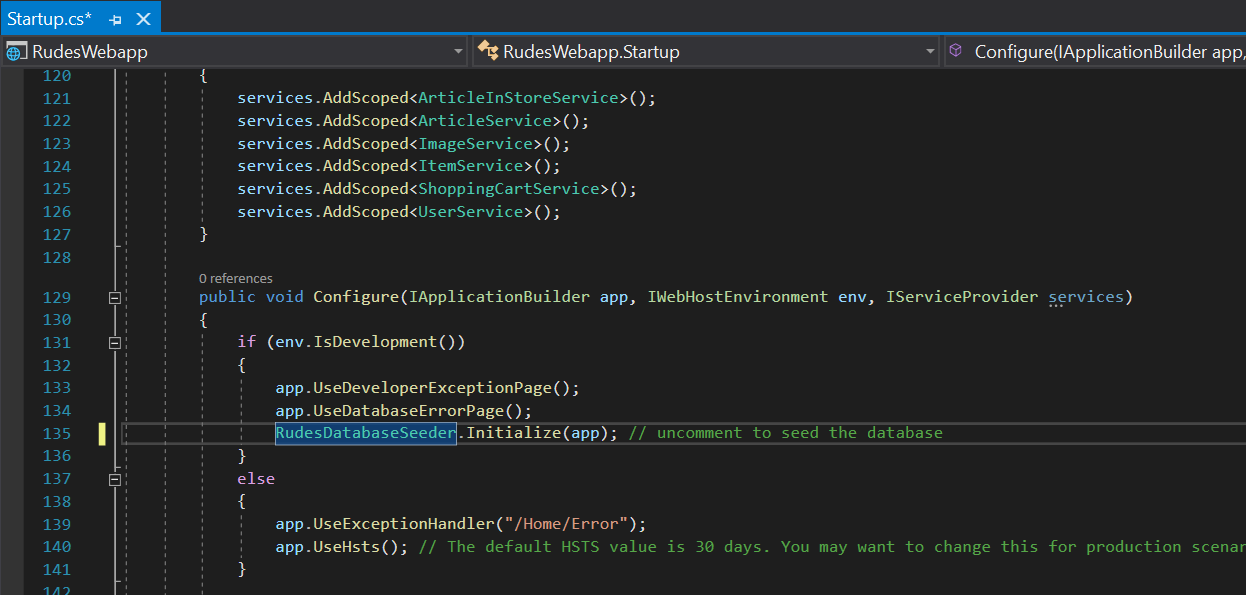
\includegraphics[width=\linewidth]{deployment/database_seeder.png}
			 	\centering
			 	\caption{Inicijalizacija Database Seeder-a}
			 	\label{fig:ClassDiagram1}
			 \end{figure}
			 
			 \textnormal{Ukoliko je došlo do promjena u bazi podataka, prije idućeg pokretanja aplikacije potrebno je u Package Manager Console pokrenuti naredbu "Update-Database" kako bi se ažurirale vrijednosti u tablicama baze. Nakon toga se aplikacija može ponovno pokrenuti.}
			 
			 \begin{figure}[H]
			 	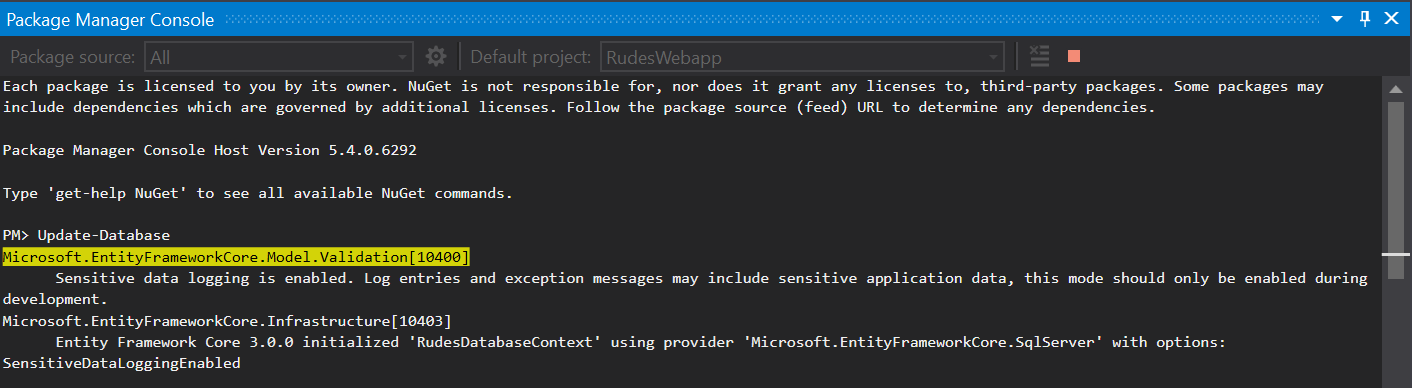
\includegraphics[width=\linewidth]{deployment/pmc_update_database.png}
			 	\centering
			 	\caption{Update-Database naredba u Package Manager Console}
			 	\label{fig:ClassDiagram1}
			 \end{figure}	
		 
		 	\textnormal{Aplikaciju smo također pustili u pogon na Azure platformi. Kao studenti imamo mogućnost besplatnog korištenja Microsoftovog programa "Azure Dev Tools for Teaching". Tamo postoji opcija dizanja vlastite web aplikacije na Azure server. Također je moguće povezati tu aplikaciju s SQL Server relacijskom bazom podataka. Obavljanjem tog postupka, dobije se link na početnu stranicu web aplikacije. Za našu stranicu link je: \href{https://rudeswebapp.azurewebsites.net/}{https://rudeswebapp.azurewebsites.net/}}.
			
			\eject 